\chapter{Introduction}		% chapter 1
\label{introchap}		% for reference (\ref{introchap})

This sample document illustrates how to use the
{\tt thesis} class, originally written by John P. Weiss
and updated by Bruce Fast.
The necessary file, \verb2thesis.cls2,
is on all the main computer systems of C.U.Boulder, 
and can be downloaded from the web site
\verb2http://www.colorado.edu/its/docs/latex/thesis/2.
Some requirements of the Graduate School are written
into that file; page size, line spacing, appropriate
placement of captions for tables and figures, etc.
Other tasks of conforming to the requirements are
left to other existing \LaTeX{} packages.
For example, a common problem is to insert graphics
--- figures and tables ---
into the body of the thesis.
For this one should use the {\tt graphicx} package,
which is part of the standard \TeX{} distribution.
Likewise, the Grad School specs say that a large
table may be displayed in landscape mode at reduced size,
but its caption must also be in rotated position,
in the same font and size as the normal text
in the body of the thesis.
To accomplish this, the user must invoke the
{\tt rotating} package,
the use of which is illustrated
in this document.
See Table \ref{tbl:sidewaysT}
and Fig. \ref{fig:sidewaysF}.


More illustrations of the use of
\verb2\label{}2 and \verb2\ref{}2:
see \S\ref{ss}
and \S\ref{sss}.
You might enjoy
\S\ref{mathchapter}			% ...see \label{mathchapter}
more than
\S\ref{introchap}.
And undoubtedly you will like
\S\ref{sec:end}				% in ch2.tex
better than either
\S\ref{sec:cata},			% in ch2.tex
Table \ref{tbl:sample3},		% in ch2.tex
or equation (\ref{eq:centerline}).	% in ch2.tex

\medskip
\section{Example of included image}

\begin{figure}[htbp]
  \begin{center}
    \leavevmode
\setlength{\unitlength}{3947sp}%
\begingroup\makeatletter\ifx\SetFigFont\undefined%
\gdef\SetFigFont#1#2#3#4#5{%
  \reset@font\fontsize{#1}{#2pt}%
  \fontfamily{#3}\fontseries{#4}\fontshape{#5}%
  \selectfont}%
\fi\endgroup%
\begin{picture}(3924,1074)(1714,-2773)
\thinlines
\put(1726,-2761){\framebox(3900,1050){}}
\put(4801,-2011){\line(-1,-6){ 61.432}}
\put(4742,-2380){\line( 2,-1){335.200}}
\put(5076,-2550){\line( 1, 1){264}}
\put(5340,-2286){\line(-1, 2){167.600}}
\put(5170,-1952){\line(-6,-1){368.595}}
\put(2026,-1861){\line( 1, 0){1875}}
\put(3901,-1861){\line(-6,-1){1641.892}}
\put(2251,-2086){\line( 1, 0){2325}}
\put(1876,-2536){\framebox(150,375){}}
\put(2251,-2386){\makebox(0,0)[lb]{\smash{\SetFigFont{12}{14.4}{\rmdefault}
	{\mddefault}{\updefault}Saved as a \LaTeX{} figure??}}}
\end{picture}
    \caption{A \LaTeX{} ``figure'', using {\tt $\backslash$framebox}}
    \label{fig:latexfig}
  \end{center}
\end{figure}
Figure \ref{fig:combustion} shows something or other;
the image is from a PostScript file which is
imported into this document using the \verb2graphicx2 package
(notice that the \LaTeX{} command
\verb2\usepackage{graphicx}2 appears
near the very top of the main \LaTeX{} file)
and the \verb2\includegraphics{...}2 command.


\begin{figure}[htbp]
  \begin{center}
    \leavevmode
 %   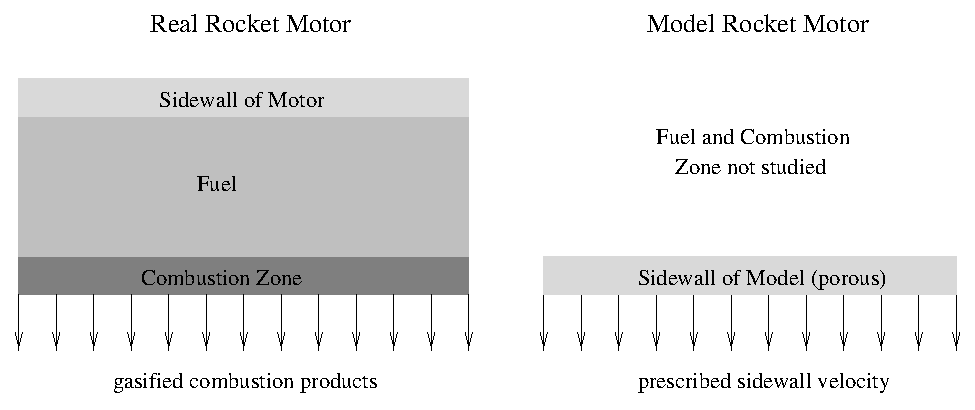
\includegraphics[width=130mm]{figures/comb.eps}
    \caption[A figure imported from a PostScript file]{
	The combustion zone in a rocket motor chamber is
	thin relative to the radius of the chamber, etc.
	How did this image get into the thesis?
	I used the {\tt $\backslash$includegraphics}
	command, which is defined in the {\tt graphicx} package.
	(The ``sub-captions'' are part of the PostScript image.)}
    \label{fig:combustion}
  \end{center}
\end{figure}


\begin{singlespacing}
\subsection{Use of $\backslash${\tt includegraphics}:}
\noindent Use
\indent \verb2\includegraphics[2\emph{options}\verb3]{figX.eps}3\\
or
\indent \verb2\includegraphics*[2\emph{options}\verb3]{figX.eps}3,\\
where the starred form clips the image so that nothing outside
the image bounding box will appear in the document.
The options include any of the following, in any order,
separated by commas:
\begin{itemize}
\item \verb9bb=llx lly urx ury9 ~ ~ -- bounding box coordinates,
	overriding any in the image file itself
\item \verb9angle=9\emph{angle} ~ ~ -- in degrees, counterclockwise
\item \verb9width=9\emph{width} ~ ~ -- specify units, e.g., {\tt 85mm}
\item \verb9height=9\emph{height} ~ ~ -- specify units, e.g., {\tt 60mm}
\item \verb9scale=9\emph{factor} ~ ~ -- e.g., 0.5 = half-size
\item \verb9clip=9\emph{true/false} ~ ~ -- {\tt clip=true} is
	equivalent to using the starred version
\item \verb9draft=9\emph{true/false} ~ ~ -- {\tt draft=true} inserts a
	correctly-sized blank rectangle
\end{itemize}

\noindent Additionally, you can insert the \verb9\includegraphics9
command within one of these commands;
\begin{itemize}
\item \verb9\scalebox{h_scale}[v_scale]{9\emph{text}\verb9}9
	~ -- \verb9v_scale9 is optional
\item \verb9\resizebox{h_length}{v_length}{9\emph{text}\verb9}9
	~ -- optionally use \verb9!9 for one of the lengths
\item \verb9\reflectbox{9\emph{text}\verb9}9
	~ -- reflects the contents horizontally
\item \verb9\rotatebox{angle}{9\emph{text}\verb9}9
	~ -- alternative to using \verb9\angle=9 option (above)
\end{itemize}
\end{singlespacing}


\subsection{Question:  What are the issues in studying this subject?}

A major goal in studying solid fuel rocket motors is to create a model
of the dynamics of a motor chamber.  This involves two major goals:
the combustion zone and the acoustic zone. Figure \ref{fig:combustion}
shows this.  The combustion zone consists of the thin layer above the
solid fuel where the gasification of the fuel takes places.  The zone
is very reactive and highly turbulent.  The acoustic-vortical zone is
the volume of gas above the combustion zone.  Within this zone, the
gas is non-reactive and contains acoustic waves and vorticity.


\section{Lists in {\tt thesis} class}

In {\tt thesis} class (for Colorado University),
lists are defined so that nested lists will be
numbered or marked appropriately.
First, an itemized (non-enumerated) list
prefaces each item with a bullet.
Nested itemized list use asterisks,
then dashes, then dots.
These lists are typed between
the \verb2\begin{itemize}2
and \verb2\end{itemize}2
commands.

\begin{itemize}
  \item{} This is ``itemized'' item A.
  \item{} This is ``itemized'' item B.
  \item{} This is ``itemized'' item C.
  \begin{itemize}
    \item{} This is ``itemized'' subitem A.
    \begin{itemize}
      \item{} This is ``itemized'' subsubitem A.
      \begin{itemize}
        \item{} This is ``itemized'' subsubsubitem A.
      \end{itemize}
      \item{} This is ``itemized'' subsubitem B.
    \end{itemize}
    \item{} This is ``itemized'' subitem B.
  \end{itemize}
  \item{} This is ``itemized'' item D.
\end{itemize}

Enumerated lists use the commands
\verb2\begin{enumerate}2 and
\verb2\end{enumerate}2,
and nested enumerations appear like this.

\begin{enumerate}
  \item{} This is ``enumerated'' item A.
  \item{} This is ``enumerated'' item B.
  \item{} This is ``enumerated'' item C.
  \begin{enumerate}
    \item{} This is ``enumerated'' subitem A.
    \begin{enumerate}
      \item{} This is ``enumerated'' subsubitem A.
      \begin{enumerate}
        \item{} This is ``enumerated'' subsubsubitem A.
      \end{enumerate}
      \item{} This is ``enumerated'' subsubitem B.
    \end{enumerate}
    \item{} This is ``enumerated'' subitem B.
  \end{enumerate}
  \item{} This is ``enumerated'' item D.
\end{enumerate}


The work presented
here\footnote{Footnotes are handled neatly by \LaTeX.}
is an extension of Lao\cite{lao:thesis}
and Lao et~al.\cite{lao:paper}
The driving frequency is on the order of the inverse
of the axial acoustic time scale, $t_A'= L'/C_0'$,
where $L'$ is the length of the cylinder
and $C_0'$ is the reference speed of
sound.\footnote{Remember the
traditional method of calculating the distance of lightning?
See the flash, count seconds until you hear the thunder,
divide by five, that's the number of miles.
That assumes $C_0=\frac{1 mi.}{5 s}$.}
Radial and azimuthal
velocities\footnote[5]{gratuitous footnote}
are found to vanish exponentially fast in the
downstream direction,
as suggested by Table \ref{powertable}.


\begin{table}[htb]
\label{powertable}
\caption[Example of a table with its own footnotes]{
	Here is an example of a table with its own footnotes.
	Don't use the $\backslash${\tt footnote} macro if you
	don't want the footnotes at the bottom of the page.
	Also, note that in a thesis the caption goes
	\emph{above} a table, unlike figures.
	}
\begin{center}
\begin{tabular}{||l|c|c|c|c||} \hline
	& $S$ & $P$ &   $Q^{\ast}$  & $D^{\dagger}$ \\	% footnote symbols!
	wave form & (kVA) & (kW) & (kVAr) & (kVAd) \\  \hline \hline
	Fig.  \ref{fig:latexfig} & 25.87 & 25.83 & 1.3 & $\approx 0$ \\ \hline
	Fig.  \ref{fig:combustion}a  & 25.48 & 25.00 & -2.82 & 4.03 \\ \hline
	Fig.  \ref{fig:combustion}b  & 25.11 & 18.02 & -9.75 & 14.52 \\ \hline
	Table \ref{tbl:sample2}  & 24.98 & 22.26 & 9.19 & 6.64 \\ \hline
	Fig.  \ref{tbl:sidewaysT}  & 23.48 & 15.00 & 6.59 & 16.82 \\ \hline
	Fig.  \ref{fig:pyramid}  & 24.64 & 22.81 & -0.44 & 9.3 \\ \hline
	Fig.  \ref{fig:sidewaysF}  & 23.03 & 18.01 & 3.36 & 13.95 \\ \hline
	\end{tabular}
   \\ \rule{0mm}{5mm}
   ${}^\ast$kVAr means reactive power.		% footnote symbol
\\ ${}^\dagger$kVAd means distortion power.	% footnote symbol
\end{center}
\end{table}


These results provide an analytical explanation of those
found from computational analysis by Fabnis
et~al.\cite{fabnis}  The non-axisymmetric flow near the
endwall contains cross-sectional velocity patterns that
include flow across the cylinder axis.  A viscous boundary
layer adjacent to the sidewall and near the endwall is
studied to find the transition between the transient core
flow and the no-slip condition on the sidewall.
It is found, as in Lao et~al.\cite{lao:paper}, that the
azimuthal component of the vorticity is proportional to
the inverse of the Mach number.  In addition, the axial
component of the vorticity driven by the non-axisymmetric
boundary condition at the endwall is also found to be
proportional to the the inverse of the Mach number.


